%! TEX root = ./master.tex
\lecture[Geometrische Verteilung. Lineare Kongruenzgeneratoren (LCGs). Knuth. Simulation von Zufallsvariablen, Zufallspermutationen und der geometrischen Verteilung. Empirischer Mittelwert. Erwartungswert.]{Mo 26 Apr 2021 10:17}{LCG's, Erwartungswert}


\subsubsection{Die geometrische Verteilung}
\begin{itemize}
    \item Seien $E_1,E_2,\ldots$ unabhängige Ereignisse mit
        \[
        \begin{split}
            &\mathbb{P}(E_i \text{ tritt ein}) = 1-q \\
            &\mathbb{P}(E_/ \text{ tritt nicht ein}) = q
        \end{split}
        .\] 
\end{itemize}
Wir verwenden wieder \tikz \fill[blue] circle (2pt); um das Eintreteten eines Ereignisses zu notieren, und \tikz \fill[red] circle (2pt); für das Gegenteil. \\
\noindent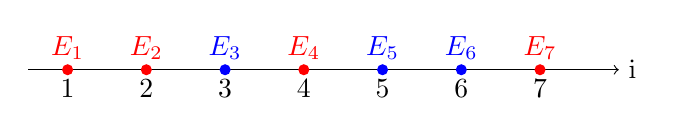
\begin{tikzpicture}
    \draw[->] (0.5,0) -- (8,0) node[anchor=west] {i};
    \foreach \x in {1,2,4,7} {
        \fill[red] (\x,0) node[anchor = north,black]{$\x$} node[anchor=south] {$E_{\x}$} circle (2pt);
    }
    \foreach \x in {3,5,6} {
        \fill[blue] (\x,0) node[anchor = north,black]{$\x$} node[anchor=south] {$E_{\x}$} circle (2pt);
    }
\end{tikzpicture} \\
\noindent Setze nun $T_0 =0$ sowie $T_{l+1} = \min \left \{i>T_l\colon E_i \text{ tritt ein}\right\} $ als die Eintrittszeitpunkte des  $k$-ten Erfolgs. Dann definieren
\[
    N_l := T_l - T_{l-1} - 1 = \# \left \{\tikz \fill[red] circle (2pt); \text{ zwischen } T_{l-1} \text{ und } T_{l}\right\} 
.\] 
die Abstände zwischen den jeweiligen Erfolgen. Es ergibt sich:
\begin{equation}
    \begin{split}
        \mathbb{P}(N_l = k) &= \mathbb{P}(N_1=k) = \mathbb{P}(T_1 = k+1)  \\
                            &= \mathbb{P}\left( \bigcap_{i=1} ^k \left \{E_i \text{ tritt nicht ein}\right\}   \cap  \left \{E_{k+1} \text{ tritt ein}\right\}\right) \\
                            &= \left(\prod_{i=1}^{k} \mathbb{P}(E_i \text{ tritt nicht ein}) \right) \cdot \mathbb{P}(E_{k+1} \text{ tritt ein}) \\
                            &=(1-q)q^k
    \end{split}
\end{equation}
    für $k\geq 0$. Das motiviert nun
    \begin{definition}[Geometrische Verteilung]\label{def:geometrische-verteilung}
        Sei  $q\in [0,1)$. Die Wahrscheinlichkeitsverteilung auf $\left \{0,1,2,\ldots\right\} $ mit Massenfunktion
        \[
            p(k) = (1-q)q^k
        .\] 
        heißt \vocab[Verteilung!geometrische]{geometrische Verteilung} mit Parameter $q$.
    \end{definition}
    \begin{notation}
        Wir notieren hierfür $\Geo(q)$
    \end{notation}
    \begin{warning}
        Eine andere Version setzt $p(k) = (1-q)q^{k-1}$, wobei $k=1,2,\ldots$. Hier ist nur der Index verschoben. Wenn nicht anders genannt, ist für uns aber immer obige Definition gemeint.
    \end{warning}
\subsection{Simulation von Gleichverteilung}
\label{sec:simulation-von-gleichverteilung}
\begin{question}
    Wie werden Zufallsvariablen simuliert?
\end{question}
\underline{Typischerweise} benutzen wir folgende Situation:
\begin{description}
    \item[Input] Zahl(en), z.B. Redinerzeit
    \item[Output] 'Zufällige Zahl' in $\left \{0,\ldots,m-1\right\} $
\end{description}

\subsubsection{Lineare Kongruenzgeneratoren (LCG)}
\begin{description}
    \item[Startwert] $x_0\in \N$ gegeben.
    \item[Parameter] $a,c,m\in \N$
    \item[Schritt] Setze $x_{n+1} := (a\cdot x_n + c) \mod m$.
\end{description}
Dieses Vorgehen produziert eine scheinbar zufällige Folge.
\begin{example}
    Es gibt folgende LCGs: \\
        \begin{tabular}{r|c|c|c}
            & m & a & c \\
            {\sc zx81} & $2^{16}+1$ & 75 & 0 \\
            {\sc randn} &  $2^{31}$&$65539$  & 0\\
            Marsaglia & $2^{32}$ & $69069$ & 1
        \end{tabular}
\end{example}
\begin{example}[Eine schlechte Wahl]
    Wenn wir $a=4, c=1, m=31$ wählen sowie  $x_0 = 3$,  so erreichen wir Periode 9, und somit werden nicht alle Zahlen erreichen / generieren. 
\end{example}
    \todo{Plot einfügen}

\begin{lemma}[Knuth]\label{lm:knuth}
    Die Periode eines LCG ist gleich $m$, genau dann, wenn
     \begin{enumerate}[label=\protect\circled{\alph*}]
        \item $c$ und  $m$ haben keine gemeinsamen Primfaktoren
        \item Jeder Primfaktor von  $m$ ist ein Teiler von  $a-1$ 
        \item Falls $4 \mid m$, dann $4 \mid  a-1$.
    \end{enumerate}
\end{lemma}
\begin{proof}
    Kein Beweis.
\end{proof}
\todo{Beispiele von LCG's einfügen}

\subsubsection{Zufallsvariablen aus $[0,1)$}
 \begin{itemize}
     \item Sei $(x_n)_{n\geq 1}$ eine Folge von (Pseudo)zufallszahlen aus $\left \{0,1,\ldots,m-1\right\} $. Dann ist
         \[
             u_n := \left(\frac{x_n}{m}\right)_{n\geq 1}
         .\] 
         eine Folge von Pseudozahlen in $[0,1)$. Gut ist aber nur der Fall, wenn $m\approx 10^N$, wobei $N=$ Rechnergenauigkeit, d.h. $\#\text{Ziffern}$.
\end{itemize}
\subsubsection{Zufallspermutationen}
\begin{question}
Wie erzugt man eine gleichverteilte Permutation von $\left \{1,\ldots,N\right\} $?
\end{question}
\begin{algorithm}[H]\label{alg:zufällige-permutation}
    \SetKwInput{KwInput}{Eingabe}
    \SetKwInput{KwOutput}{Ausgabe}
    \SetKwInput{KwLaufzeit}{Laufzeit}
    \SetKw{KwGoTo}{go to}
    \SetKwProg{Fn}{Def}{:}{}
    \DontPrintSemicolon

    \caption{Zufallspermutationen}
    \KwInput{Möglichkeit, aus endlicher Menge gleichverteilt zufällige Zahlen zu ziehen}
    \KwOutput{Eine zufällige Permutation von $\left \{1,\ldots,N\right\} $}
    \;
    Setze $\sigma_0:=\left \{1,\ldots,N\right\} $\;
    \For{$i=1$ \KwTo  $n-1$}{
    wähle $k\in \left \{i,\ldots,N\right\} $ gleichverteilt \;
    Setze $\sigma_k := \sigma_{k-1}\circ \tau_{i,k}$ \;
}
\end{algorithm}
\begin{lemma}
    Der Algorithmus erzeugt eine zufällige gleichverteilte Permutation.
\end{lemma}

\begin{proof}
    Der Algorithmus benutzt eine Gleichverteilung auf
    \[
    \Omega_n := \left \{1,\ldots,N\right\}  \times  \left \{2,\ldots,n\right\} \times \left \{n-1,n\right\} 
    .\] 
    Für $\omega = (w_1,\ldots,w_{N-1})\in \Omega_N$ ist
    \[
        \sigma(\omega) = τ_{N-1,\omega_{N-1}} \circ  \ldots \circ  \tau_{1,w} \circ  \underbrace{(1,\ldots,N)}_{\sigma_0}
    .\] 
    Es genügt also zu zeigen, dass $\sigma : \Omega_N \to  \mathcal{S}_N$ eine Bijektion ist. Wir sehen:
    \begin{enumerate}[label=\protect\circled{\alph*}]
        \item $\abs{\Omega_N} = \abs{\mathcal{S}_N} = N!  $ 
        \item Sei $w\neq \tilde{\omega} $ und setze $k = \min \left \{j \mid  \omega_j \neq  \tilde{\omega} _j\right\} $. Dann ist $σ(\omega)_k \neq  σ(\tilde{\omega} )_k$ und somit ist die Funktion injektiv
    \end{enumerate}
    Damit ist die Abbildung sogar bijektiv und wir sind fertig.
\end{proof}
\subsubsection{Geometrische Verteilung}
Sei $X \sim  \Geo(q)$, d.h.
        \[
            \mathbb{P}(X=k) = (1-q)q^k
        .\] 
        \begin{question}
        Wie simuliert man nun $X$?
        \end{question}
Erzeuge zunächst $n \sim  U[0,1)$ als gleichverteilte Zufallsvarable auf $[0,1)$. \\
Sei  $T_k:= \mathbb{P}(X<k)$. Falls $n \in [T_k, T_{k+1})$, dann setze $X = k$. Wir berechnen also
\begin{equation}
    \begin{split}
        T_k &= \mathbb{P}(X<k) = 1-\mathbb{P}(X\geq k) \\
            &= 1- \sum_{x\geq k}(1-q)q^k \\
            &= 1-q^k
    \end{split}
\end{equation}
    Wegen
    \[
        u = 1-q^x \iff  x = \frac{\ln (1-u)}{\ln (q)}
    .\] 
erhalten wir also für $k$ den Wert
 \[
     k := \left\lfloor \frac{\ln (1-u)}{\ln (q)} \right\rfloor = \left\lfloor \frac{\ln (\tilde{u})}{\ln (q)} \right\rfloor 
.\] 
wobei wir ebenfalls $\tilde{u} \sim  U[0,1)$ gleichverteilen.
\subsection{Erwartungswert und Varianz}
\begin{itemize}
    \item Sei $X$ eine  \underline{reellwertige} diskrete Zufallsverteilung. Sei 
        \[
        X : \Omega \to  \mathcal{S}\subset \R
        .\] 
        eine diskrete Zufallsvariable, d.h. $\mathcal{S}$ abzählbar.
\end{itemize}
\begin{definition}[Empirischer Mittelwert]\label{def:empirischer-mittelwert}
    Seien $x_1,\ldots,x_n\in \mathcal{S}$ $n$ Beobachtungen einer Zufallsvariable $X$. Der \vocab{empirische Mittelwert} ist durch
    \[
    \frac{1}{n}\sum_{i=1}^n x_i
    .\] 
    definiert.
\end{definition}
\begin{goal}
    Wir wollen eine Sorte von Mittelwert definieren, der nur von $X$ abhängig ist, und nicht von den Beobachtungen.
\end{goal}

Folgende Forderungen ergeben sich an solch einen Mittelwert:
        \begin{itemize}
            \item Falls $X(\omega) = x$ für jedes $\omega$, dann muss der \underline{Mittelwert} von $X$ gleich  $x$ sein. 
            \item Jeder Wert $x\in \mathcal{S}$ muss bezüglich der Massenfunktion $p_X(x)$ gewichtet sein.
        \end{itemize}
        Das motiviert folgende
        \begin{definition}[Erwartungswert]\label{def:erwartungswert}
    Der \vocab{Erwartungswert} von $X$ bzgl.  $\mathbb{P}$ ist durch
    \[
        \mathbb{E}(X) = \sum_{s\in \mathcal{S}} s\cdot \mathbb{P}(X=s) = \sum_{s\in \mathcal{S}} s\cdot p_{X}(s)
    .\] 
    definiert. Dies ist wohldefiniert, falls die Reiche absolut gegen einen Wert $<\infty$ konvergiert.
\end{definition}
Stellen wir uns $\mathcal{S}$ als Balken vor und tragen an den stellen $s_i \in \mathcal{S}$ jeweils das Gewicht $m_i := p_X(s_i)$ an, so ist  $\mathbb{E}(X)$ derjenige Punkt, mit dem der Balken ausbalanciert ist: \\
\vspace{1em}
\begin{tikzpicture}
    \draw[->] (0,0) -- (6,0) node[anchor=west] {$\mathcal{S}$};
    \newcommand{\ball}[3]{\fill[blue] (#1,0) circle (#2pt) node[anchor=south] {{\tiny $m_#3$}} node[anchor=north,black] {$s_#3$}; \draw[red,->] (#1,0) -- (#1,-0.3*#2);}
    \ball{1}{2.5}{1}
    \ball{2.3}{1}{2}
    \ball{2.9}{1.8}{3}
    \ball{5}{3}{4}
    \draw[->,red,thick] (3.2,-1) node[anchor=north]{$\mathbb{E}(X)$}-- (3.2,0);
\end{tikzpicture}
\begin{remark}
    Nicht alle Wahrscheinlichkeitsverteilungen besitzen einen endlichen Mittelwert, das zeigt folgendes
\end{remark}
\begin{example}
    Sei $X$ auf  $\left \{1,2,\ldots\right\} $ verteilt mit
    \[
        \mathbb{P}_X(s) = \frac{6}{\pi^2\substack{r} }
    .\] 
    dann ergibt sich für den Erwartungswert:
    \[
        \mathbb{E}(X) = \sum_{s\geq 1} s\cdot \frac{6}{\pi^2s^2} = \frac{6}{\pi^2} \cdot  \sum_{s\geq 1} \frac{1}{s}\to  \infty
    .\] 
\end{example}





